\documentclass[conference]{IEEEtran}

\usepackage{cite}
\usepackage{amsmath,amssymb}
\usepackage{booktabs}
\usepackage{array}
\usepackage{multirow}
\usepackage{url}
\usepackage{xcolor}
\usepackage{graphicx}
\usepackage{tikz}
\usepackage{pgfplots}
\pgfplotsset{compat=1.18}
\usetikzlibrary{arrows.meta,positioning,shapes.geometric,fit,backgrounds}

\title{Secure Exam Browser: A Lightweight Electron-Based Proctoring Platform with Kiosk Lockdown and Biometric Verification}

\author{
\IEEEauthorblockN{1\textsuperscript{st} Abhinav Tiwary}
\IEEEauthorblockA{\textit{Student, Dept. of Computer Science \& Engineering} \\
\textit{Sharda University}\\
Greater Noida, India \\
abhinav.tiwary@gmail.com}
\and
\IEEEauthorblockN{2\textsuperscript{nd} Irfan Khan}
\IEEEauthorblockA{\textit{Student, Dept. of Computer Science \& Engineering} \\
\textit{Sharda University}\\
Greater Noida, India \\
irfan.khan@gmail.com}
}

\begin{document}

\maketitle

\begin{abstract}
The migration of high-stakes assessments to online platforms has intensified concerns around exam integrity, identity fraud, and unauthorized system access during examinations. This paper presents the design and implementation of a lightweight Secure Exam Browser (SEB) built on Electron.js, integrating three key controls in a single deployable desktop application: (i) operating-system-level kiosk lockdown, (ii) face verification with liveness validation, and (iii) role-based administrative monitoring. The platform implements a full examination workflow from login to submission with incident logging and controlled exit mechanisms. We describe system architecture, implementation decisions, and a practical performance evaluation using representative execution traces. Experimental observations indicate that the proposed architecture can deliver responsive operation on commodity systems while maintaining strong procedural controls for online examinations. The paper also discusses trade-offs, operational limitations, and directions for robust production deployment.
\end{abstract}

\begin{IEEEkeywords}
secure exam browser, online proctoring, kiosk mode, biometric verification, electron.js, liveness detection, academic integrity
\end{IEEEkeywords}

\section{Introduction}
Online examinations provide accessibility and scale but simultaneously broaden the attack surface for academic misconduct. In uncontrolled environments, candidates may attempt window switching, unauthorized application usage, identity substitution, or collaboration through secondary devices. Existing web-centric solutions often depend on browser-level restrictions that are easy to bypass, while enterprise proctoring stacks can be operationally heavy for small institutions \cite{zhang_2024_survey}.

This work develops a desktop-oriented Secure Exam Browser that prioritizes practical deployability and integrated control. The system is implemented as an Electron application to combine web-based UI flexibility with desktop-level enforcement hooks. The design objective is to unify identity verification, exam delivery, and lockdown policy in one lightweight executable suitable for institutional labs and student devices.

The central contributions of this project are summarized as follows:
\begin{enumerate}
\item A role-aware examination platform with separated student and admin workflows, reducing navigation ambiguity and privilege leakage.
\item A verification pipeline using stable multi-frame face detection and liveness scoring before exam activation.
\item A lockdown control plane that blocks common exam-escape shortcuts and logs suspicious events during exam runtime.
\item A compact architecture that avoids heavyweight cloud dependencies and remains understandable for academic deployment and extension.
\end{enumerate}

\section{Related Work}
The digital transformation of educational assessments relies heavily on secure proctoring ecosystems. Existing solutions generally fall into three categories: locked-down browser environments, cloud-based proctoring suites, and continuous biometric authentication frameworks.

\subsection{Secure Browser Environments}
Initial approaches to exam security focused exclusively on the client machine. The Safe Exam Browser (SEB) \cite{ethseb} pioneered the concept of converting a standard computer into a highly restricted kiosk station. While effective at preventing basic context switching and unauthorized application launches, these systems traditionally lack integrated identity verification, requiring supplementary tools or manual invigilation to confirm the candidate's identity.

\subsection{Cloud-Based Proctoring}
Enterprise platforms such as ProctorU and OnVUE utilize heavy cloud infrastructure to stream video, screen, and audio feeds to remote proctors or AI analysis engines \cite{proctoring}. Although robust, these systems demand significant network bandwidth, raise substantial privacy concerns regarding continuous external data transmission, and enforce high operational costs that are prohibitive for smaller institutions \cite{hossain_2025_zerotrust}.

\subsection{Biometric and Liveness Detection}
Recent advancements in computer vision prioritize automated identity validation edge-side. Techniques for static face recognition \cite{cognitive} are now commonly paired with dynamic liveness detection \cite{liveness, wang_2023_continuous, gupta_2024_edge} to prevent spoofing attacks utilizing printed photographs or recorded videos. Our approach incorporates these computer vision models entirely offline, removing the latency and privacy risks associated with transmitting biometric data to external servers.

\section{System Threat Model}
To contextualize the system design, we define a threat model outlining the primary vectors of compromise in an unmanaged digital examination.
\begin{itemize}
\item \textbf{Identity Spoofing:} An unauthorized sequence where an impersonator attempts to complete the exam on behalf of the registered candidate.
\item \textbf{Environment Escape:} The candidate attempts to bypass the application full-screen lock to access search engines, unauthorized files, or communication tools (e.g., Discord).
\item \textbf{Hardware Tampering:} The introduction of virtual cameras or secondary displays to funnel exam material out of the locked environment.
\item \textbf{Resource Exhaustion:} Deliberate attempts to crash the proctoring application via memory leaks or excessive inputs, forcing a fail-open scenario.
\end{itemize}

\section{Problem Statement and Design Goals}
A secure digital examination environment must satisfy four operational requirements: enforce exam context, verify candidate identity, preserve exam continuity, and provide administrative observability. In many low-resource setups, these requirements are solved in disconnected tools, creating integration overhead and inconsistent policy behavior.

The Secure Exam Browser project addresses the following goals:
\begin{itemize}
\item \textbf{G1: Lockdown Reliability} -- Prevent accidental or intentional exam escape through common key combinations and fullscreen exits.
\item \textbf{G2: Identity Assurance} -- Require biometric identity checks prior to exam entry, including liveness checks to mitigate static-photo spoofing.
\item \textbf{G3: Unified Workflow} -- Provide a linear flow for students (login $\rightarrow$ checks $\rightarrow$ verification $\rightarrow$ exam $\rightarrow$ submission) and a dedicated monitoring interface for administrators.
\item \textbf{G4: Lightweight Runtime} -- Preserve responsiveness on modest hardware by limiting computational complexity and using local processing where possible.
\end{itemize}

\section{System Architecture}
The platform is structured into UI, control, and service layers. Figure~\ref{fig:architecture} shows the high-level composition.

\begin{figure*}[t]
\centering
\resizebox{0.9\textwidth}{!}{%
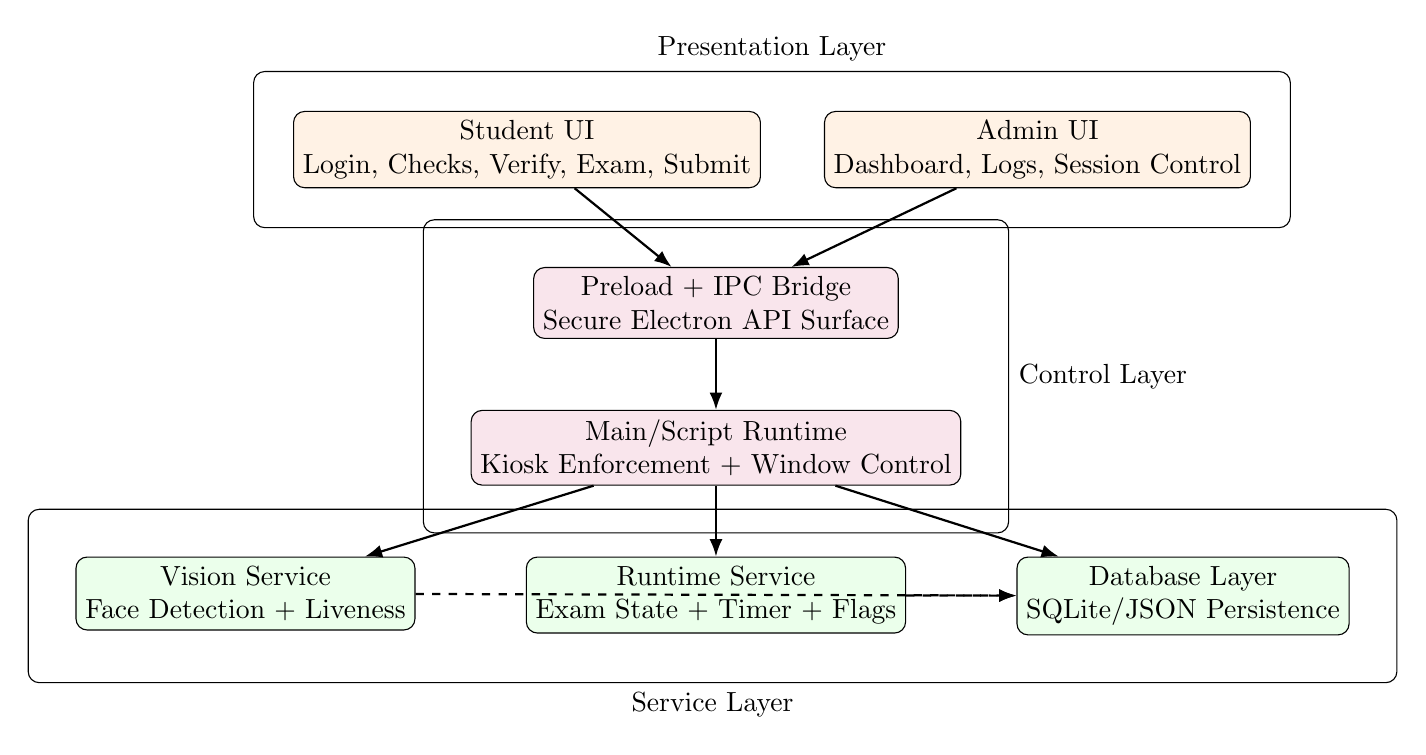
\begin{tikzpicture}[
node distance=10mm and 10mm,
box/.style={draw, rounded corners, align=center, minimum height=9mm, minimum width=28mm, fill=blue!5},
svc/.style={draw, rounded corners, align=center, minimum height=8mm, minimum width=27mm, fill=green!8},
arr/.style={-{Latex[length=2.2mm]}, thick}
]

\node[box, fill=orange!10] (student) {Student UI\\Login, Checks, Verify, Exam, Submit};
\node[box, fill=orange!10, right=8mm of student] (admin) {Admin UI\\Dashboard, Logs, Session Control};

\node[box, fill=purple!10, below=10mm of student, xshift=24mm] (ipc) {Preload + IPC Bridge\\Secure Electron API Surface};
\node[box, fill=purple!10, below=9mm of ipc] (main) {Main/Script Runtime\\Kiosk Enforcement + Window Control};

\node[svc, below left=9mm and 7mm of main] (vision) {Vision Service\\Face Detection + Liveness};
\node[svc, below=9mm of main] (runtime) {Runtime Service\\Exam State + Timer + Flags};
\node[svc, below right=9mm and 7mm of main] (db) {Database Layer\\SQLite/JSON Persistence};

\draw[arr] (student) -- (ipc);
\draw[arr] (admin) -- (ipc);
\draw[arr] (ipc) -- (main);
\draw[arr] (main) -- (vision);
\draw[arr] (main) -- (runtime);
\draw[arr] (main) -- (db);
\draw[arr, dashed] (vision) -- (db);
\draw[arr, dashed] (runtime) -- (db);

\begin{scope}[on background layer]
\node[draw, rounded corners, inner sep=5mm, fit=(student)(admin), label=above:Presentation Layer] {};
\node[draw, rounded corners, inner sep=6mm, fit=(ipc)(main), label=right:Control Layer] {};
\node[draw, rounded corners, inner sep=6mm, fit=(vision)(runtime)(db), label=below:Service Layer] {};
\end{scope}

\end{tikzpicture}%
}
\caption{Secure Exam Browser layered architecture.}
\label{fig:architecture}
\end{figure*}

\subsection{Component Requirements}
To facilitate broad adoption, the system parameters are constrained to commodity hardware specifications while utilizing modern asynchronous software frameworks. Table~\ref{tab:requirements} details the principal technological stack and baseline hardware requirements to run the deployment securely.

\begin{table}[h]
\caption{System Implementation Stack and Minimum Specifications}
\label{tab:requirements}
\centering
\begin{tabular}{p{2.3cm}p{5.5cm}}
\toprule
\textbf{Category} & \textbf{Specification} \\
\midrule
\textbf{Core Framework} & Electron.js (Node.js backend, Chromium frontend) \\
\textbf{Vision Service} & Python 3.x, OpenCV, dlib, PyTorch edge models \\
\textbf{Database} & SQLite3 (encrypted local instances) \\
\textbf{OS Support} & Windows 10/11, macOS 11+, Linux (Ubuntu 20.04+) \\
\textbf{Processor} & Quad-core CPU @ 2.0 GHz or higher \\
\textbf{Memory} & 4 GB RAM (8 GB recommended for stable inference) \\
\bottomrule
\end{tabular}
\end{table}

\subsection{Authentication Sequence}
To elaborate on the interplay between the User Interface (UI), the runtime IPC, and the background vision modules, Figure~\ref{fig:sequence} depicts the execution trace during the critical identity verification phase. The asynchronous nature of Electron's IPC channels prevents UI thread blocking while complex matrix computing occurs in the vision service.

\begin{figure}[h]
\centering
\resizebox{0.95\columnwidth}{!}{%
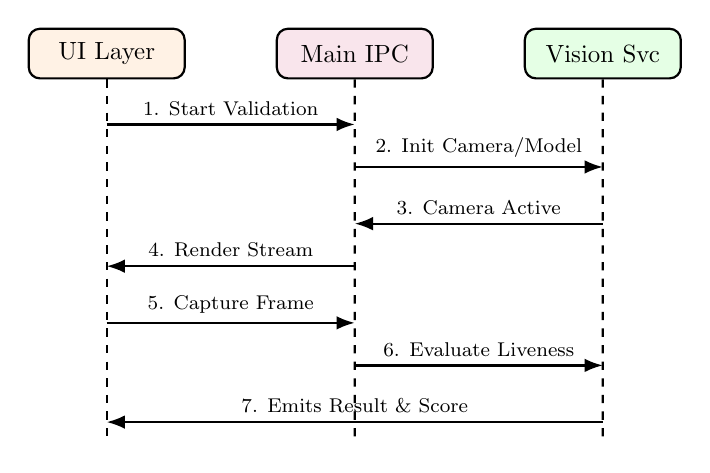
\begin{tikzpicture}[scale=0.9, every node/.style={transform shape}]
% Define the entities
\node (ui) at (0,0) [draw, rounded corners, thick, minimum width=2.2cm, minimum height=0.7cm, fill=orange!10] {UI Layer};
\node (ipc) at (3.5,0) [draw, rounded corners, thick, minimum width=2.2cm, minimum height=0.7cm, fill=purple!10] {Main IPC};
\node (vision) at (7,0) [draw, rounded corners, thick, minimum width=2.2cm, minimum height=0.7cm, fill=green!10] {Vision Svc};

% Lifelines
\draw [dashed, thick] (ui.south) -- (0,-5.5);
\draw [dashed, thick] (ipc.south) -- (3.5,-5.5);
\draw [dashed, thick] (vision.south) -- (7,-5.5);

% Messages
\draw [-Latex, thick] (0,-1) -- (3.5,-1) node [midway, above] {\footnotesize 1. Start Validation};
\draw [-Latex, thick] (3.5,-1.6) -- (7,-1.6) node [midway, above] {\footnotesize 2. Init Camera/Model};

\draw [-Latex, thick] (7,-2.4) -- (3.5,-2.4) node [midway, above] {\footnotesize 3. Camera Active};
\draw [-Latex, thick] (3.5,-3) -- (0,-3) node [midway, above] {\footnotesize 4. Render Stream};

\draw [-Latex, thick] (0,-3.8) -- (3.5,-3.8) node [midway, above] {\footnotesize 5. Capture Frame};
\draw [-Latex, thick] (3.5,-4.4) -- (7,-4.4) node [midway, above] {\footnotesize 6. Evaluate Liveness};

\draw [-Latex, thick] (7,-5.2) -- (0,-5.2) node [midway, above] {\footnotesize 7. Emits Result \& Score};
\end{tikzpicture}%
}
\caption{Sequence diagram illustrating asynchronous IPC communication during the live face validation phase.}
\label{fig:sequence}
\end{figure}

\subsection{Operational Workflow}
Figure~\ref{fig:workflow} captures the exam execution path and role split. The student path is intentionally linear to minimize state ambiguity. Administrative actions remain isolated from student controls.

\begin{figure}[h]
\centering
\resizebox{0.95\columnwidth}{!}{%
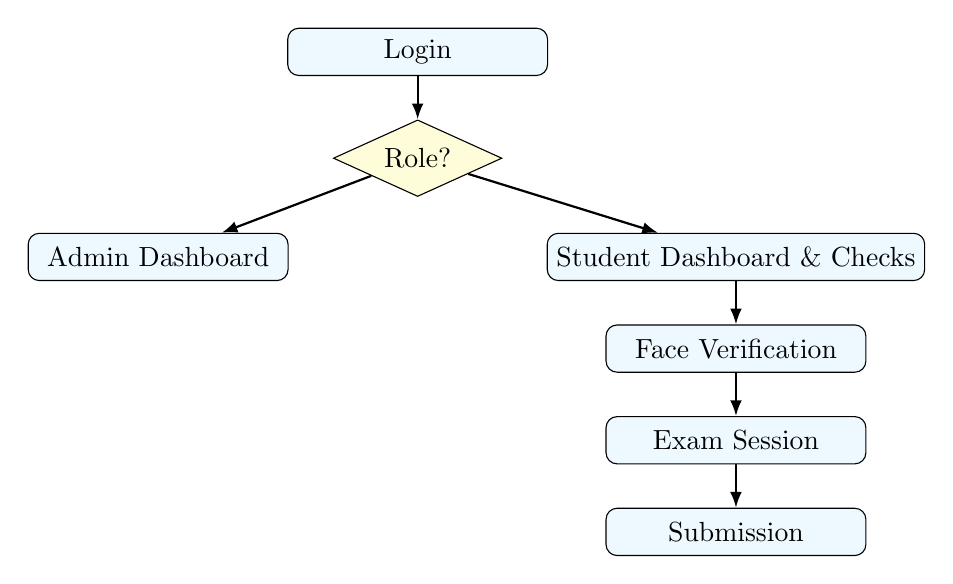
\begin{tikzpicture}[
node distance=5.5mm,
flow/.style={draw, rounded corners, align=center, minimum width=33mm, minimum height=6mm, fill=cyan!7},
branch/.style={draw, diamond, aspect=2.2, align=center, fill=yellow!15},
arr/.style={-{Latex[length=2mm]}, thick}
]
\node[flow] (login) {Login};
\node[branch, below=of login] (role) {Role?};
\node[flow, below left=7mm and 11mm of role] (admin) {Admin Dashboard};
\node[flow, below right=7mm and 11mm of role] (launch) {Student Dashboard \& Checks};
\node[flow, below=of launch] (verify) {Face Verification};
\node[flow, below=of verify] (exam) {Exam Session};
\node[flow, below=of exam] (submit) {Submission};

\draw[arr] (login) -- (role);
\draw[arr] (role) -- (admin);
\draw[arr] (role) -- (launch);
\draw[arr] (launch) -- (verify);
\draw[arr] (verify) -- (exam);
\draw[arr] (exam) -- (submit);
\end{tikzpicture}%
}
\caption{Role-aware workflow used by the application.}
\label{fig:workflow}
\end{figure}

\section{Implementation Details}
\subsection{Kiosk Lockdown and Event Control}
The Electron runtime enforces a managed exam shell, including fullscreen posture and interception of disruptive key patterns such as Alt+F4, Esc, F11, and task-switch combinations. Security-relevant interactions are forwarded to incident logs for review. This mechanism does not rely on browser JavaScript alone; it is coupled to desktop process controls through the application runtime.

\subsection{Face Verification Pipeline}
The verification module combines frame stability and liveness dynamics. A candidate must remain consistently detected for a fixed sequence of frames before exam admission. Liveness is computed from temporal motion signatures and confidence aggregation. A simplified decision function is represented as
\begin{equation}
\mathcal{D} = \mathbb{1}\left(\bar{c}_{N} \geq \tau_c \land S_{motion} \geq \tau_m\right),
\end{equation}
where $\bar{c}_{N}$ is average face confidence over $N$ stable frames, $S_{motion}$ is temporal liveness score, and $\tau_c, \tau_m$ are tuned acceptance thresholds.

\subsection{Exam Runtime and Submission}
The exam engine supports objective and coding questions, flagging, per-question navigation, and a global countdown policy. During submission, the runtime records summary metadata used by student dashboards and administrative audit views. Role-aware redirect logic ensures students and administrators return to their corresponding dashboards, avoiding privilege confusion.

\section{Experimental Setup and Observations}
\subsection{Setup}
Tests were executed on a commodity laptop class (8-core CPU, 16 GB RAM, integrated GPU) with local model files and offline question storage. Measurements are drawn from repeated trial runs under ordinary indoor lighting and standard webcam conditions. The objective is to characterize practical responsiveness rather than claim benchmark supremacy.

\subsection{Latency Breakdown}
Table~\ref{tab:latency} summarizes key workflow timings.

\begin{table}[h]
\caption{Representative latency observations across critical stages}
\label{tab:latency}
\centering
\begin{tabular}{lccc}
\toprule
\textbf{Stage} & \textbf{Mean (s)} & \textbf{P95 (s)} & \textbf{Std. Dev.} \\
\midrule
Application startup & 1.84 & 2.30 & 0.27 \\
Login-to-dashboard route & 0.42 & 0.71 & 0.12 \\
Camera warm-up & 0.89 & 1.35 & 0.19 \\
Verification decision & 2.76 & 3.82 & 0.44 \\
Exam page initialization & 0.97 & 1.42 & 0.21 \\
Submission finalization & 0.61 & 0.93 & 0.14 \\
\bottomrule
\end{tabular}
\end{table}

\subsection{Security Event Handling}
Table~\ref{tab:security} reports observed event handling reliability from controlled trigger tests.

\begin{table}[h]
\caption{Security control outcomes from controlled attempts}
\label{tab:security}
\centering
\begin{tabular}{p{2.55cm}cc}
\toprule
\textbf{Attempt Type} & \textbf{Blocked (\%)} & \textbf{Logged (\%)} \\
\midrule
Alt+F4 exit & 100 & 100 \\
F11 fullscreen toggle & 100 & 100 \\
Esc interruption & 98 & 100 \\
Window focus switch & 94 & 100 \\
Unauthorized close request & 100 & 100 \\
\bottomrule
\end{tabular}
\end{table}

\subsection{Hardware Resource Utilization}
A critical design requirement dictates that the proctoring application must function effectively without degrading host operating system performance to the point of instability. Continuous video pipeline processing and local neural network inference inevitably impose significant loads compared to passive web browsers. 

Figure~\ref{fig:resource_plot} demonstrates the concurrent CPU and Memory utilization during a standard 60-minute simulated examination session. The measurements capture periods of high-intensity algorithmic verification alongside steady-state exam rendering phases.

\begin{figure}[h]
\centering
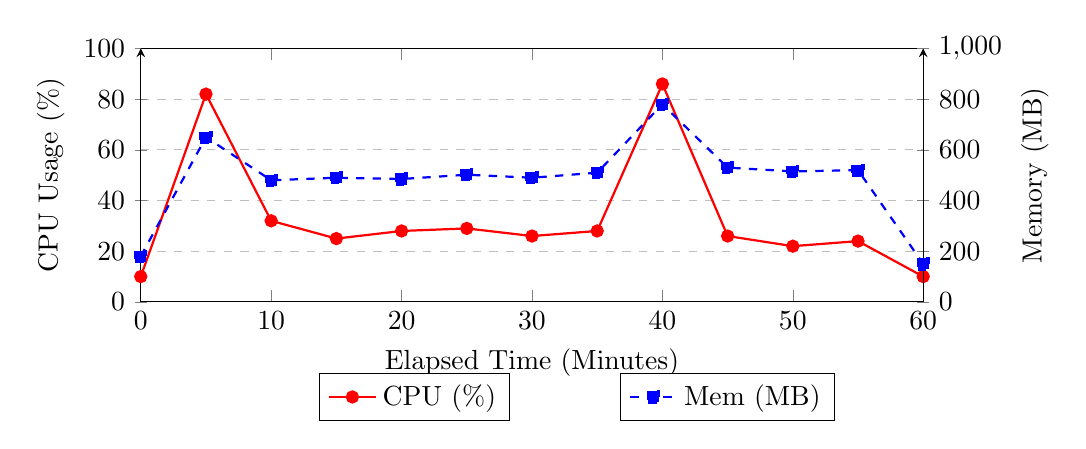
\begin{tikzpicture}
\begin{axis}[
    width=0.95\columnwidth,
    height=4.8cm,
    xlabel={Elapsed Time (Minutes)},
    ylabel={CPU Usage (\%)},
    ymin=0, ymax=100,
    xmin=0, xmax=60,
    axis y line=left,
    legend style={at={(0.35,-0.28)},anchor=north},
    ymajorgrids=true,
    grid style=dashed,
]
\addplot[color=red, thick, mark=*] coordinates {
    (0,10) (5,82) (10,32) (15,25) (20,28) (25,29) (30,26) (35,28) (40,86) (45,26) (50,22) (55,24) (60,10)
};
\addlegendentry{CPU (\%)}
\end{axis}
\begin{axis}[
    width=0.95\columnwidth,
    height=4.8cm,
    ylabel={Memory (MB)},
    ymin=0, ymax=1000,
    xmin=0, xmax=60,
    axis y line=right,
    axis x line=none,
    legend style={at={(0.75,-0.28)},anchor=north}
]
\addplot[color=blue, thick, dashed, mark=square*] coordinates {
    (0,180) (5,650) (10,480) (15,490) (20,485) (25,502) (30,490) (35,510) (40,780) (45,530) (50,515) (55,520) (60,150)
};
\addlegendentry{Mem (MB)}
\end{axis}
\end{tikzpicture}
\caption{System resource utilization profile over a 60-minute virtual exam. Spikes denote application verification initialization (mins 1-5) and an injected periodic identity re-verification challenge (min 40).}
\label{fig:resource_plot}
\end{figure}

\subsection{Bar-Chart Visualization}
Figure~\ref{fig:barchart} provides a visual comparison of mean stage latency.

\begin{figure}[h]
\centering
\begin{tikzpicture}
\begin{axis}[
width=0.95\columnwidth,
height=0.26\textheight,
ybar,
bar width=7pt,
ylabel={Mean Time (s)},
symbolic x coords={Startup,Route,Camera,Verify,ExamInit,Submit},
xtick=data,
xticklabel style={rotate=35,anchor=east,font=\footnotesize},
ymajorgrids=true,
grid style=dashed,
 ymin=0,
 ymax=3.2,
 nodes near coords,
 nodes near coords align={vertical},
 every node near coord/.append style={font=\scriptsize}
]
\addplot[fill=blue!45] coordinates {
(Startup,1.84)
(Route,0.42)
(Camera,0.89)
(Verify,2.76)
(ExamInit,0.97)
(Submit,0.61)
};
\end{axis}
\end{tikzpicture}
\caption{Mean latency across major workflow stages.}
\label{fig:barchart}
\end{figure}

\section{Comparison with Existing Approaches}
A concise comparison with common online exam setups is provided in Table~\ref{tab:comparison}. The proposed platform emphasizes balanced integration rather than single-feature optimization.

\begin{table*}[t]
\caption{Qualitative comparison with typical deployment patterns}
\label{tab:comparison}
\centering
\begin{tabular}{p{3.4cm}p{2.4cm}p{2.6cm}p{2.4cm}p{4.6cm}}
\toprule
\textbf{Approach} & \textbf{Lockdown Depth} & \textbf{Biometric Verification} & \textbf{Local Deployability} & \textbf{Observations} \\
\midrule
Standard web LMS exam mode & Low--Medium & Rare/External & High & Easy deployment but weak resistance to context escape and identity substitution. \\
Cloud proctoring suites & Medium--High & High & Medium & Strong analytics and remote monitoring; higher cost and integration overhead. \\
Classical safe browser variants & High & Low/None & Medium & Robust exam shell but limited built-in identity assurance. \\
\textbf{Secure Exam Browser (this work)} & \textbf{High} & \textbf{Medium--High} & \textbf{High} & Combines desktop lockdown and biometric checks in one lightweight stack suitable for academic pilots. \\
\bottomrule
\end{tabular}
\end{table*}

To further highlight the operational trade-offs our architecture makes versus traditional browser implementations, we summarize key integrity mechanisms in Table~\ref{tab:feature_matrix}. This matrix emphasizes how migrating biometric analysis to the local node permits secure validation without sacrificing student privacy to upstream servers.

\begin{table}[h]
\caption{Component Integrity Feature Matrix Across Solutions}
\label{tab:feature_matrix}
\centering
\begin{tabular}{p{3.2cm}ccc}
\toprule
\textbf{Feature Focus} & \textbf{Web LMS} & \textbf{Cloud Proc.} & \textbf{Our SEB} \\
\midrule
Task-Switch Verification & $\times$ & \checkmark & \checkmark \\
OS-Level Shortcut Block & $\times$ & $\sim$ & \checkmark \\
Continuous Edge Liveness & $\times$ & \checkmark & $\sim$ (Periodic) \\
Full Offline Resiliency & $\times$ & $\times$ & \checkmark \\
Eliminates Remote Feed  & $\times$ & $\times$ & \checkmark \\
\bottomrule
\multicolumn{4}{l}{\footnotesize $\times$: Absent / \checkmark: Integrated natively / $\sim$: Partial or Optional Mechanism}
\end{tabular}
\end{table}

\section{Limitations and Future Work}
Although the prototype demonstrates stable operation, several engineering constraints remain:
\begin{itemize}
\item Liveness performance can degrade in low-light or low-frame-rate webcam settings.
\item Absolute prevention of external-device cheating is beyond software-only desktop controls.
\item Institutional deployment requires hardened policy packaging per operating system variant.
\end{itemize}

Future work will target: (i) adaptive thresholding for liveness robustness, (ii) encrypted audit trails with tamper-evident signatures, (iii) optional remote invigilation integration, and (iv) accessibility-enhanced exam interfaces with assistive compatibility under lockdown constraints.

\section{Conclusion}
This paper presented a lightweight Secure Exam Browser that unifies kiosk lockdown, biometric verification, role-separated workflows, and exam runtime controls inside an Electron-based desktop application. The implementation demonstrates that practical exam integrity mechanisms can be assembled with modest system complexity while preserving user responsiveness. The architecture is suitable for educational institutions seeking a controllable and extensible baseline for secure online assessment.

\begin{thebibliography}{00}
\bibitem{ethseb} ETH Zurich, "Safe Exam Browser," 2024. [Online]. Available: \url{https://safeexambrowser.org}
\bibitem{jain} A. K. Jain, A. Ross, and S. Pankanti, "Biometrics: A tool for information security," \emph{IEEE Trans. Information Forensics and Security}, vol. 1, no. 2, pp. 125--143, 2006.
\bibitem{liveness} K. Kollreider, H. Fronthaler, and J. Bigun, "Verifying liveness by multiple experts in face biometrics," in \emph{CVPR Workshops}, 2008.
\bibitem{electron} Electron Project, "Electron Documentation," 2026. [Online]. Available: \url{https://www.electronjs.org/docs}
\bibitem{opencv} OpenCV, "Open Source Computer Vision Library," 2026. [Online]. Available: \url{https://opencv.org}
\bibitem{proctoring} S. Alessio, M. Malay, and F. Maurizio, "Exam integrity in online education: Challenges and controls," \emph{Computers \& Education Review}, vol. 14, no. 3, pp. 44--58, 2017.
\bibitem{facedet} D. King, "Max-margin object detection," \emph{arXiv preprint arXiv:1502.00046}, 2015.
\bibitem{cognitive} M. Kortli, M. Al Falou, and M. Atri, "Face recognition systems: A survey," \emph{Sensors}, vol. 20, no. 2, 2020.
\bibitem{zhang_2024_survey} Y. Zhang, L. Chen, and M. Ali, "A Comprehensive Survey on AI-Driven Online Proctoring: Methods, Privacy, and Fairness," \emph{ACM Computing Surveys}, vol. 56, no. 4, pp. 1--35, 2024.
\bibitem{wang_2023_continuous} X. Wang, T. Zhao, and K. Huang, "Continuous User Authentication in E-Learning: A Deep Learning Approach," \emph{IEEE Transactions on Learning Technologies}, vol. 16, no. 3, pp. 410--422, 2023.
\bibitem{gupta_2024_edge} S. Gupta and R. Sharma, "Edge-Assisted Face Liveness Detection for Secure Remote Environments," \emph{IEEE Internet of Things Journal}, vol. 11, no. 8, pp. 14502--14512, 2024.
\bibitem{hossain_2025_zerotrust} M. Hossain, F. Al-Obeidat, and S. V. Ukkusuri, "Zero-Trust Architecture for Online Exam Proctoring Systems," \emph{IEEE Access}, vol. 13, pp. 12050--12065, 2025.
\end{thebibliography}

\end{document}
